\documentclass{article}
\usepackage{amsmath,amssymb}
\usepackage{hyperref}
\usepackage{graphicx}

\title{\bf{Laboratory Project One: Calibration of a Pressure Transducer}}
\author{Nicholas Malaya \\ Department of Mechanical Engineering \\ University of Texas at Austin} \date{}

\begin{document}
\maketitle
\date{}

This document details the calibration and uncertainty quantification of
an Omega PX164-005D5V pressure transducer. 
\newline
\newline
Lab Partners: Jon Langston \& Owen O'Neal

\newpage
\section{Presentation of Calibration Data}

\textbf{You will have calibration data from using two different
standards and at least two repeats in each case.  
Present these results appropriately. Estimate the linear curve fit from
these data and display on the figures with the data.  
Ascertain whether a linear curve fit is appropriate or whether better
accuracy could be obtained with a different curve fit. Comment about
these results, particularly on any unusual or unexpected results.}  

\subsection*{Inclined Manometer Results}

  \begin{figure}[!htb]
   \begin{center}
    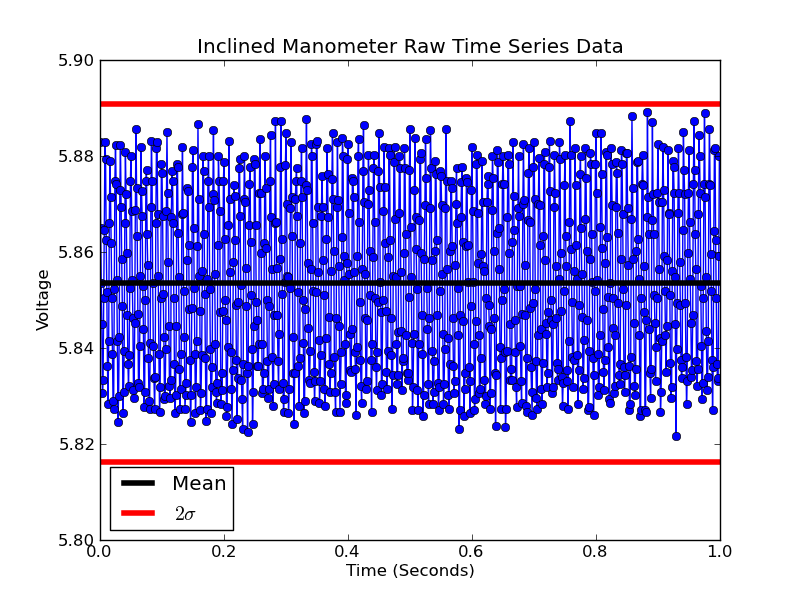
\includegraphics[width = 12 cm]{figs/incl_time.png}
    \caption{Example raw time series data from a single inclined manometer
    run. The calculated mean of the signal is shown in black, along with
    the two $\sigma$ (standard deviation) confidence interval in
    red.}
    \label{incl-time}
   \end{center}
  \end{figure}

We begin with the inclined manometer results. Figure \ref{incl-time}
depicts the voltage measured at the pressure transducer as a function of
time. One thousand samples were taken over a period of one second. This
signal was then analyzed to calculate the mean and standard deviation of
the sample, which are also depicted on the figure. These numbers appear
roughly sane, with the mean clearly near the center of the signal, and
the two $\sigma$ bands encompassing the vast majority of the points (we
would expect 95\%). Furthermore, the signal appears to be ``white
noise'', namely evenly distributed around the mean (no bias) and with
little or no correlation between samples e.g. subsequent readings of
the signal are not obviously visibly correlated with the previous step.

However, we can do better than evaluating these properties by
eyeball. Let's examine a histogram of the timeseries data, which is
shown below in Figure \ref{incl-hist}. 

  \begin{figure}[!htb]
   \begin{center}
    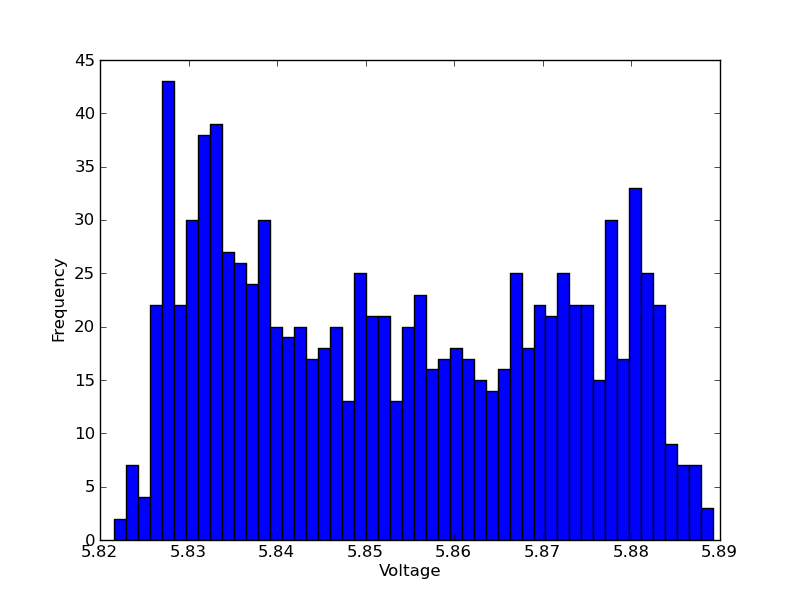
\includegraphics[width = 12 cm]{figs/incl_hist.png}
    \caption{Histogram depicting the frequency of voltages in our
    signal. This was generated with fifty bins, but the results did not
    appear to be sensitive to the number selected.}
    \label{incl-hist}
   \end{center}
  \end{figure}

Yikes. This does not look good at all. In the limit of a large number of
samples, I would have expected to see a Gaussian (due to the central
limit theorem) that is centered around the mean and smooth tails. 
Instead of a nice smooth gaussian distribution we have essentially a
uniform distribution of samples across all values. This does not make me
happy, but I'm having difficulty stating if this is certainly a problem,
instead of just a strange oddity of the data sampling. Perhaps, the
samples are more correlated with each other than they had appeared to my
eyeballs. Thankfully, we have a way to check this as well. Let's look at
the autocorrelation of the signal, to investigate this further. 

  \begin{figure}[!htb]
   \begin{center}
    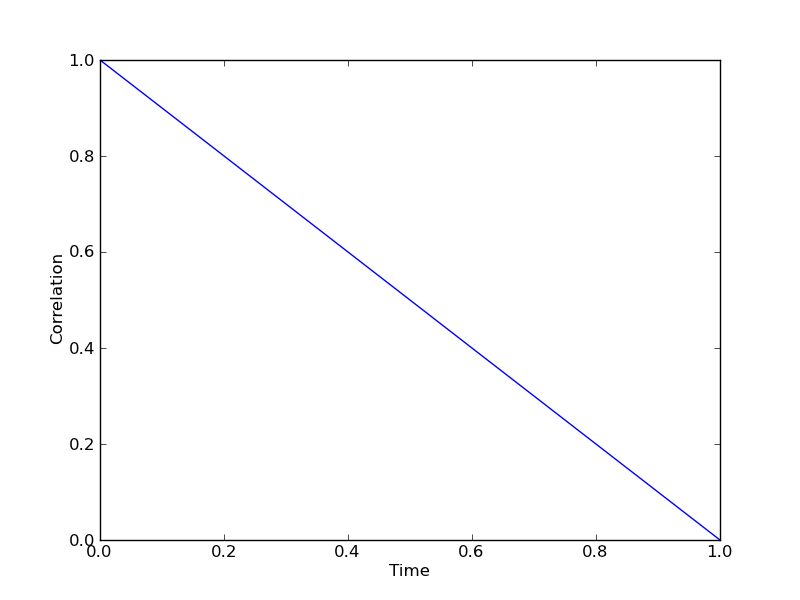
\includegraphics[width = 12 cm]{figs/incl_auto.png}
    \caption{Autocorrelation of the voltage as a function of time.}
    \label{incl-auto}
   \end{center}
  \end{figure}

When I saw this I assumed something was wrong in the matplotlib acorr()
function, and calculated this indepdently in xmgrace. Sadly, the same
result was obtained. Clearly, this data was poorly obtained. What is
wrong? The correlation of our signal does not reduce to zero until
nearly the very end of our time sampling window. For instance, at 0.8
seconds, our samples still have roughly a 20\% correlation with the
initial time sample! In other words, while I initially claimed to have
1000 samples, I have far, far fewer ``effective samples''. Our
statistics will be much more suspect as a result. 

What happened? Almost certainly we had far too high of a sampling
rate, and the samples were much more correlated in time than we had
realized. Conclusion: 1000 samples per second is far too large of a
frequency. We discussed the sampling rate during data collection, and
given the time readout of the signal (and the eyeball norm we discussed
above) nothing seemed to be out of place. It has only been during this
data analysis step that serious irregularities have appeared. 

You go to war with the data you have, so let's proceed. The next step is
to calculate a mean and standard deviation for each sample, plot this
and then perform a linear regression of the best fit line through this
dataset. This is shown below, in Figure \ref{inclined}. 

  \begin{figure}[!htb]
   \begin{center}
    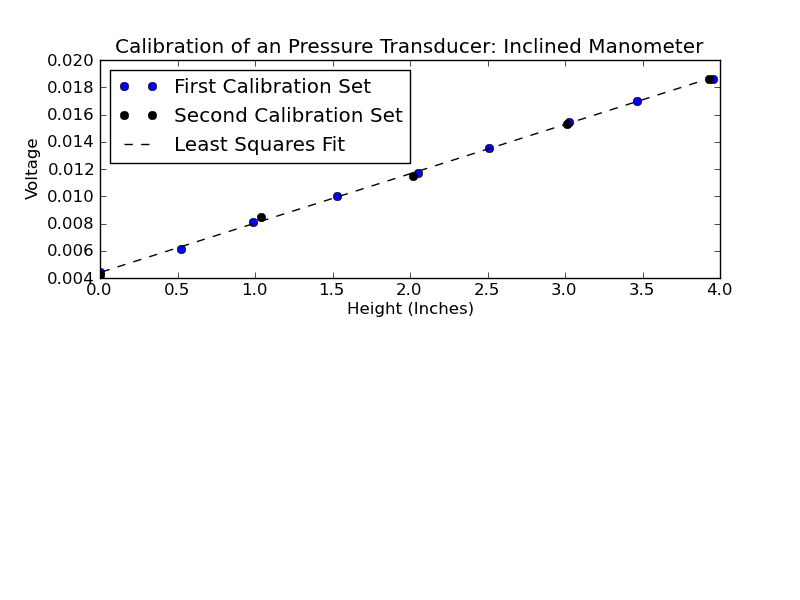
\includegraphics[width = 12 cm]{figs/inclined.png}
    \caption{Scatter plot of the averaged time samples for both
    calibration runs, along with a dotted line depicting the Least
    Squares Fit.}
    \label{inclined}
   \end{center}
  \end{figure}

We attempted to mix things up between calibration runs, by changing the
location of the calibration points (in height of column of water) as
well as by changing the human operator of the inclined manometer (from
intially Jon to Owen). As one can see from the plot, these changes did
not materially impact the calibration data point readings, and therefore
did not have substantial impact on the prediction of the linear
fit. This speaks favorable towards the repeatability of the calibration.

The
linear fit is also quite good. The $R^2 =$ 0.999552862197, which implies
an extremely tight fit (99.9\%) between the data and the prediction resulting
from the linear fit. In fact, I find this goodness of fit slightly
suspicious, as it is too high. I wonder if we made this, ``too easy'' by
using large variations in the column of water height (from 4.0 to 0.0)
and if we got lucky with out small statistical sample size (from
earlier) not introducing large deviations from the true mean. 

Nevertheless, with an $R^2$ value that high, and given the trend in the
data, I feel confident stating that our data implies a linear
relationship between the height of the column of water and the voltage
produced at the transducer. While higher order fits (polynomials, etc.)
will always improve the goodness of fit, they will also introduce
spurrious oscillations and are more prone to over-fit. I see no reason
to believe that a higher order fit is appropriate, given these
results. I believe this data constitutes a ``validation'' of the
transducers linear response. 

Of course, I would be hesitant to use the transducer outside of the
calibration regime shown here. It is entirely possible that our
calibration data fell into a linear response range, and that
extrapolations outside this range will fail due to a non-linear response
in voltage from the transducer.


\subsection*{Micro-Manometer Results}

I don't believe it is necessary to discuss these results in as great
detail as before, but I'll provide a similar overview. Suffice to say,
this is plagued by similar over-sampling results. In Figure
\ref{micro-time}, we can again see that while the fluctuations are
larger, the signal output has a similar character. 

  \begin{figure}[!htb]
   \begin{center}
    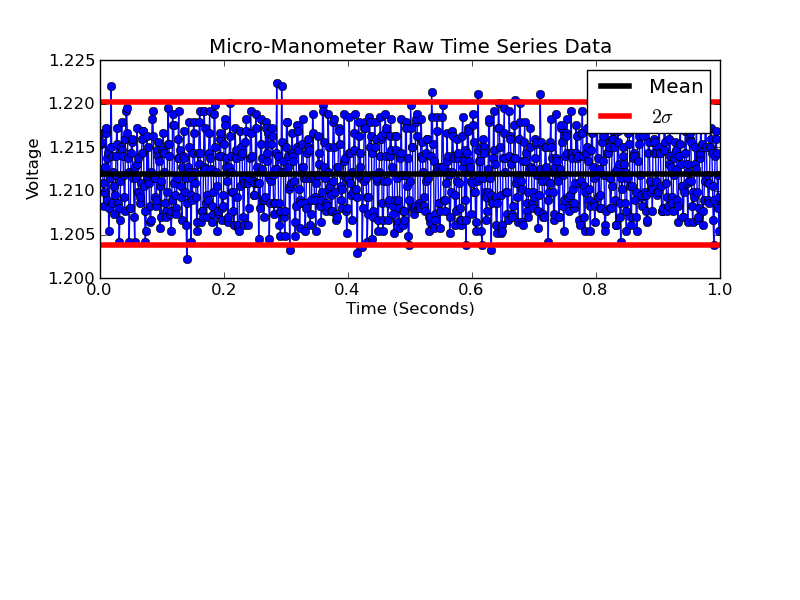
\includegraphics[width = 12 cm]{figs/micro_time.png}
    \caption{Example raw time series data from a single micro-manometer
    run. The calculated mean of the signal is shown in black, along with
    the two $\sigma$ (standard deviation) confidence interval in
    red.}
    \label{micro-time}
   \end{center}
  \end{figure}

The histogram (shown in Figure \ref{micro-hist}) appears cleaner, with
at least tails of a distribution dropping away from the mean but again
does not provide a great deal of confidence that our samples are truly
independent. 
  \begin{figure}[!htb]
   \begin{center}
    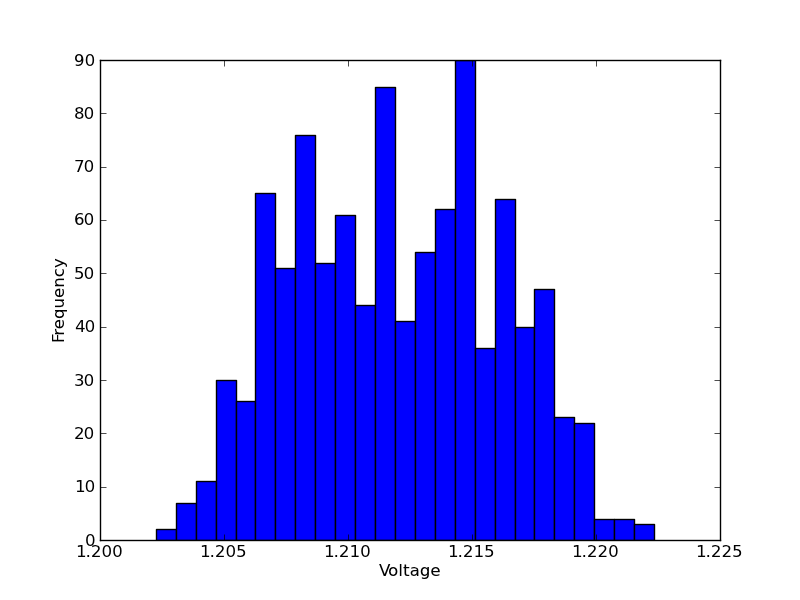
\includegraphics[width = 12 cm]{figs/micro_hist.png}
    \caption{Histogram depicting the frequency of voltages in our
    signal. This was generated with fifty bins, but the results did not
    appear to be sensitive to the number selected.}
    \label{micro-hist}
   \end{center}
  \end{figure}

Figure \ref{random} displays a plot of the autocorrelation 1000 samples
of synthetic data. These are 1000 synthetic data samples that were
randomly generated numbers. This plot is included to demonstrate two
things:  
\begin{itemize}
 \item What a more reasonable autocorrelation would appear as.
 \item Evidence the software is functioning properly.
\end{itemize}

  \begin{figure}[!htb]
   \begin{center}
    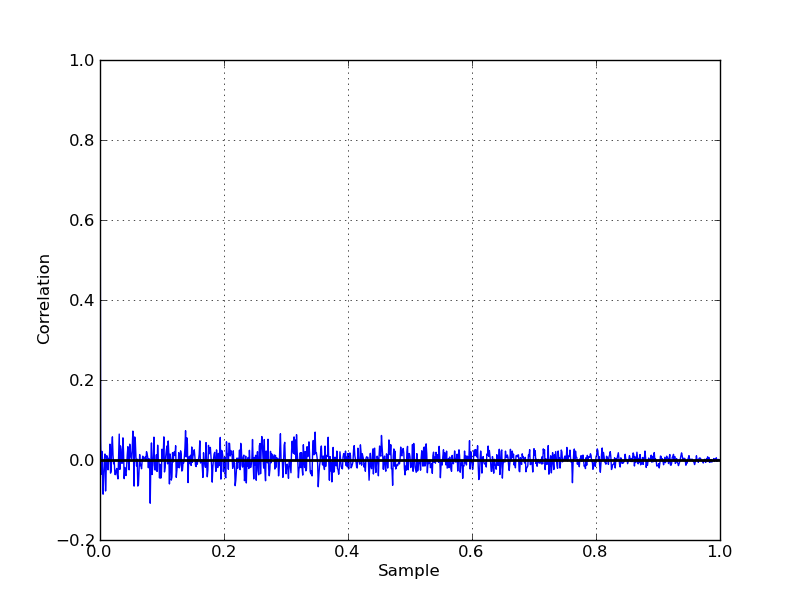
\includegraphics[width = 12 cm]{figs/random.png}
    \caption{The autocorrelation of 1000 samples that were randomly
    generated numbers.}
    \label{random}
   \end{center}
  \end{figure}

As it should, the correlation drops from 1 at $t=0$ (which can barely be
seen on the plot) quickly into ``the
noise'' near a correlation of zero. I would expect well sampled data
(e.g. nearly independent) to appear much more like this plot. Needless
to say, the micro-manometer data also appears to be over-sampled. 

  \begin{figure}[!htb]
   \begin{center}
    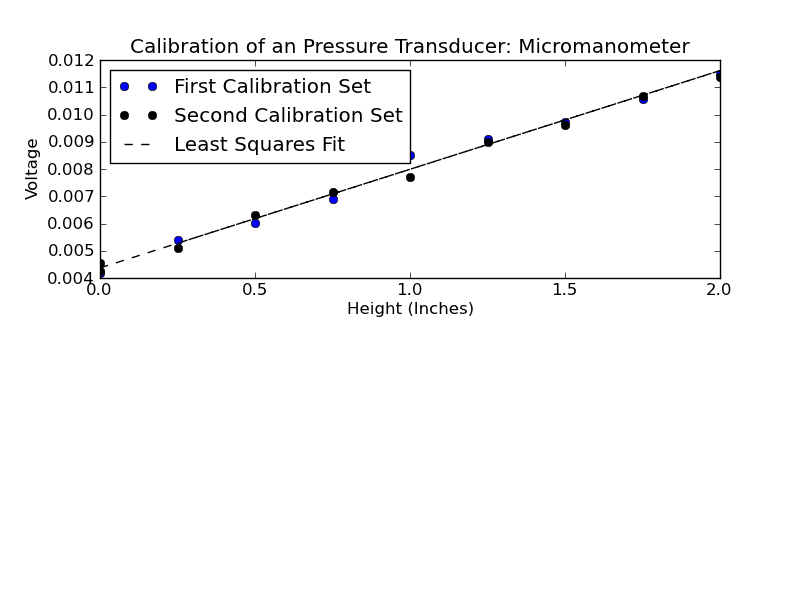
\includegraphics[width = 12 cm]{figs/micro.png}
    \caption{Scatter plot of the averaged time samples for both
    calibration runs, along with a dotted line depicting the Least
    Squares Fit.}
    \label{micro}
   \end{center}
  \end{figure}


Figure \ref{micro} shows the plot and least squares best fit line. 
This scatter plot has an $R^2 =$ 0.990071511099, which again is an
excellent fit. As before, the results appear to be largely reproducable,
as the second calibration set is certainly highly consistent with the
first, despite again slightly changing the location of measurement as
well as the operator of the apparatus (from Jon to Owen, again). I
should note that these runs were all logged using the labview software
by Nick, so that element remains ironclad and consistent across runs. 

\newpage
\section{Uncertainty Analysis}

\textbf{Estimate the uncertainty of the pressure measurements with the
pressure transducer using the linear curve fit you have determined in
your calibration. Compare this with the manufacturer's specifications of
an accuracy. Also estimate the lowest pressure differential that you can
measure with at least $\pm 10\%$ accuracy. Be sure to justify these
estimates with analyses.}

We now calculate the error bounds on each datum individually, using the formula, 
\begin{equation}
  \delta \hat Y = t_{0.05} * S_{y,x} \left[ \frac{1}{n} + \frac{x^2}{\Sigma x^2} \right]
\end{equation}

Here, $S_{y,x}$ is the standard error of fit, defined as, 
\begin{equation}
  S_{y,x}^2 = \frac{\Sigma (Y-\hat Y)^2}{n-2}
\end{equation}
and $t_{0.05}$ is the 95\% confidence interval bound estimated from the data. 
We replace this with the two $\sigma$ value, as for a Gaussian distribution 
(expected to result in data that is independent and with sufficient sample 
size, due to the central limit theorem). In other words, 
\begin{equation}
  t_{0.05} = 2 \sigma.
\end{equation}



The results of this error estimate are shown in Figure \ref{error-incl} 
for the inclined manometer, and  Figure \ref{error-micro} for the micro-manometer.

\begin{figure}[!htb]
  \begin{center}
    \includegraphics[width = 12 cm]{figs/error-incl.png}
    \caption{Linear Regression alongside the error estimates for the inclined manometer. }
    \label{error-incl}
  \end{center}
\end{figure}

\begin{figure}[!htb]
  \begin{center}
    \includegraphics[width = 12 cm]{figs/error-micro.png}
    \caption{Linear Regression alongside the error estimates for the micro-manometer. }
    \label{error-micro}
  \end{center}
\end{figure}

%% The forward propagation of uncertainty will be performed here the
%% ``Standard technique'' of Moffat. In general, this applies to
%% functionals of the form, 
%% \begin{equation}
%%   R_0 = f(x_1,x_2, \ldots ,x_N)
%% \end{equation}
%% Where the individual contribution is of each variable to uncertainty is,
%% \begin{equation}
%%   \delta R_i = \frac{\partial R_0}{\partial x_i} \delta x_i
%% \end{equation}
%% and the total uncertainty may be calculated as, 
%% \begin{equation}
%%   \delta R_0 = \left(\delta R_1^2 + \delta R_2^2 + \ldots + \delta R_N^2 \right)^{1/2}
%% \end{equation}
%% However, we implicitly assume a linear fit of the form, 
%% \begin{equation}
%%   V = m*x_1 + b. 
%% \end{equation}
%% This implies our functional is a function of only one variable, $\Delta p$, 
%% \begin{equation}
%%   R_0 = f(x_1)
%% \end{equation}
%% and therefore,
%% \begin{equation}
%%   \delta R_0 = \left(\delta R_1^2 \right)^{1/2} = \delta R_1 =
%%    \frac{\partial R_0}{\partial x_1} \delta x_1.
%% \end{equation}
%%  Notice however that we can evaluate this partial derivative, 
%% \begin{equation}
%%  \frac{\partial R_0}{\partial x_1} \delta x_1 = \frac{\partial}{\partial
%%   x_1}\left( m*x_1 +b \right) \delta x_1 = m \delta x_1. 
%% \end{equation}
%% In words, this means that the uncertainty of our voltage prediction can
%% be calculated as the uncertainty measured in the heights multiplied by
%% the slope of the best fit line. The smallest units of measurement were
%% .01 for the inclined and .001 for the micro. We can likely measure these
%% by another half, by assessing the height of the column between these two
%% keys. As a result, we will estimate $\delta x_1$ for the inclined and
%% micro as .005 and .0005, respectively. The slopes, m, for these cases
%% are 0.0036191 (inclined) and 0.0036178 (micro). Thus, the products, $m
%% \delta x_1$ will be: 
%% \begin{eqnarray}
%% 1.80955e-05 \text{ Volts} & (\text{inclined}) \\
%% 1.80890e-06 \text{ Volts} & (\text{micro}). 
%% \end{eqnarray}




\subsection{Estimate the Lowest Pressure Differential You Can Measure
  with at least 10\% Accuracy}

Our model for the pressure differential utilizes the Bernoilli equation
(and all its accompanying assumptions) for a fluid with no velocity that
differs only by height. As a result, the equation has the form,
\begin{equation}
 \rho g \Delta h = \Delta P. 
 \label{bern}
\end{equation}
We have previously established that the smallest height that can be
measured is .005 and .0005 for the inclined and micro cases. Values of
height changes below these thresholds will presumably have 100\% error,
as no adjustment to the estimated value will be logged. The change in
height that would result in only 10\% error must therefore be 10x the
size of the smallest height change measurable, or .05 and .005. We can
then apply these height changes to equation \ref{bern} using $rho$ for
H20 at STP (977.8 kg/$m^3$) and g at the surface of the earth (9.81 m/s)
to arrive at our estimates of the smallest pressure gradient we can
measure, which are: 
\begin{eqnarray}
 479.1 \text{ Pascals} & (\text{inclined}) \\
 47.91 \text{ Pascals} & (\text{micro}). 
\end{eqnarray}

It is difficult for me to estimate if this is a reasonable
answer. Atmospheric pressure is 101,325 Pascals, so the micro-manomter would in
principle be able to detect .047\% changes in pressure near sea-level, which sounds
small but not implausible. If we imagine this working as a static tube,
then using,
\begin{equation}
V = \left(\frac{2 \Delta P}{\rho}\right)^{1/2}
\end{equation}
we would be able to estimate changes in velocity as small as 0.313 m/s,
which certainly seems reasonable, and perhaps larger than I would have
expected. 

\end{document}
